\documentclass[main.tex]{subfiles}

\pagestyle{fancy}
\fancyhf{}
\fancyhead[LE]{\makebox[\pageoffset][l]{\bfseries\thepage}\bfseries\leftmark}
\fancyhead[RO]{\bfseries\rightmark\makebox[\pageoffset][r]{\bfseries\thepage}}

\begin{document}

\section*{Goal}
Today we will investigate the Work-Energy Theorem by measuring the work done on an object as well as the change in kinetic energy of the object. We will also investigate the conservation of energy as we turn potential energy into kinetic energy.

\section*{Equipment}
\begin{itemize}
\item
850 Universal Interface
\item
PASCO Capstone Software
\item
Force Sensor, Photogate with Pulley, Photogate
\item
Dynamics track, cart, end stop for track
\item
Cart-mountable picket fence
\item
Stand for Force Sensor
\item
String
\item
Masses, mass hanger
\item
Triple-beam Balance
\item
Phillips screwdriver
\end{itemize}•

\section*{Theory}
For an object with mass $m$ that experiences a force parallel $F_{||}$ to its displacement $\mathbf{x},$ the work done on the object is,
\begin{equation} \label{eq:WorkDef}
W=F_{||}x=Fx\cos{\theta}=\mathbf{F}\cdot\mathbf{x}.
\end{equation}
In our experiments, we will assume that $F$ and $\theta$ (the angle between the directions of $\mathbf{F}$ and $\mathbf{x}$) are constant; also we will assume that $\mathbf{F}$ and $\mathbf{x}$ will be in the same direction, thus simplifying Equation \eqref{eq:WorkDef} to,
\begin{equation} \label{eq:Work_Simplified}
W=Fx.
\end{equation}

Using Newton's Second Law and one of the kinematic equations, or a little calculus, we can develop what is called the Work-Energy Theorem,
\begin{equation}\label{eq:WET}
W=\Delta KE=KE_{f}-KE_{i}=\frac{1}{2}mv_{f}^2-\frac{1}{2}mv_{i}^2.
\end{equation}
This will be left as an exercise in lab.

When studying springs, it is often helpful to use Hooke's Law,
\begin{equation}\label{eq:Hooke}
\mathbf{F}=-k\mathbf{x},
\end{equation}
which describes the force on the end of a spring that has been displaced (compressed or stretched) a distance $x.$ (The minus sign implies that the force always points back toward the spring's equilibrium position.) The spring constant $k,$ can be determined experimentally by applying different forces to compress or stretch the spring to different distances. Then if we were to plot the applied force versus the distance, the slope of our graph would be $k.$

This spring force is a conservative force, meaning that it has a potential energy associated with it. The elastic potential energy of a spring is given by,
\begin{equation}\label{eq:PE_Spring}
PE_{spring}=\frac{1}{2}kx^2.
\end{equation}•
If the energy is conserved, i.e., if there are no losses, such as friction, then any decrease in the elastic potential energy in the compressed spring will be completely converted into kinetic energy when the spring pushes against an object of mass $m.$

\section{Setup I: Work-Energy Theorem}
For this activity, the force sensor measures the force applied to the cart by a string that is suspended over a pulley with an object of known mass at the end of the string. The Photogate Pulley measures the motion of a cart as it is pulled. Capstone will display the force applied, and the distance and speed of the object. The program integrates the area under a curve of force versus distance to determine the work done. (Equation~\eqref{eq:Work_Simplified} treats the simple case where $F$ is constant during the whole displacement. Calculus teaches how to extend Equation~\eqref{eq:Work_Simplified} to the case of a varying force by the process called ``integration" which is the same as calculating an area.) The program calculates the final kinetic energy. The final kinetic energy is compared to the work done.
\begin{enumerate}
\item
Start Capstone
\item
Connect the Force Sensor and Photogate Pulley to the 850UI.
\item
Open the file titled ``Energy1" by clicking on 
\includegraphics{Open_Experiment}. The file should be located in ..\textbackslash Documents\textbackslash Phys Lab Files\textbackslash Phys1154.
\item
Measure and record the mass of both the cart and the Force Sensor.
\item
Use a \#0 Phillips head screwdriver to mount the Force Sensor onto the accessory tray of the cart.
\item
Put adjustable feet on both ends of the track. Using the feet, adjust the height to level the track so that cart will not roll one way or another.
\item
Put one end stop at the end of the track and place the cart next to the end stop.
\item
Mount the Photogate with Pulley on the end of the track so that the top edge of the pulley is approximately the same height as the hook on the Force Sensor that is mounted on top of the cart.

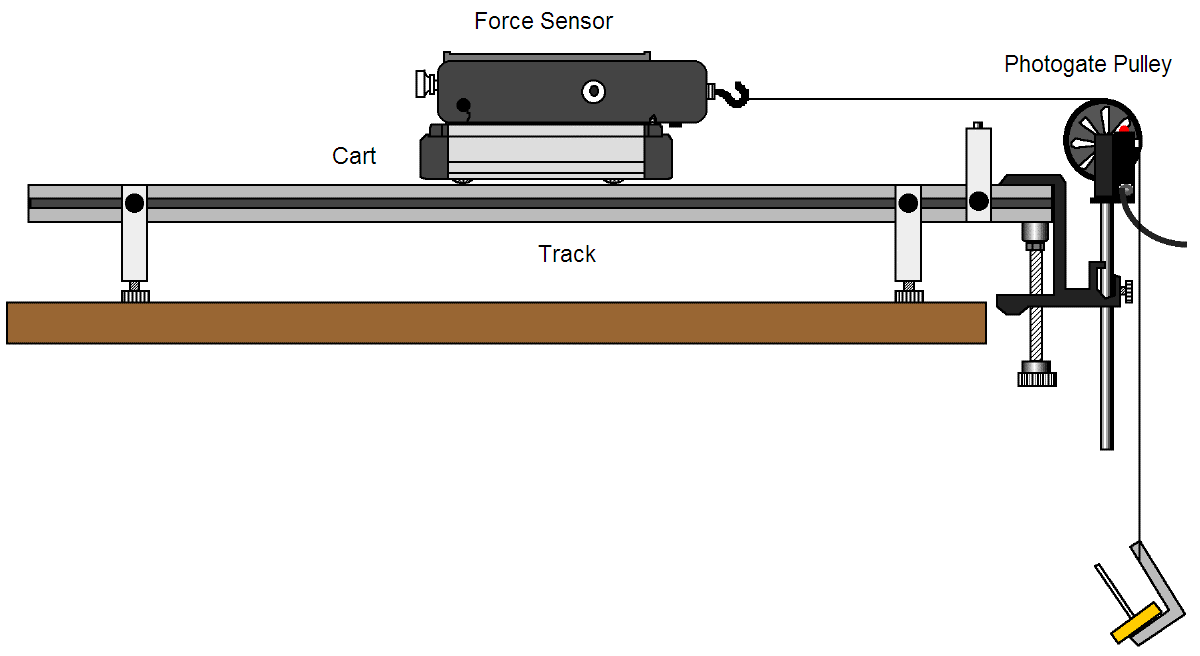
\includegraphics[width=\textwidth]{Energy_1_Setup}

\item
In Capstone, click on ``Calibration." We will use a two-standard calibration for the Force Sensor.
\item
For the first calibration point, press the tare button on the side of the force sensor to zero the sensor. Type in 0 N for the standard value and click ``Set Current Value to Standard Value."
\item
Use a piece of string that is about 10 cm longer than the distance from the top of the Photogate Pulley to the floor. Connect one end of the string to the Force Sensor's hook and hang the string over the Photogate Pulley.
\item
Attach an object of known mass $m$ to the end of the string so that the bottom of the object is just above the floor when the end of the cart is against the end stop.
\item
Enter the object's weight in Newtons as the second calibration point as a \emph{positive} value and click ``Set Current Value to Standard Value."
\item
Press ``Next" then ``Finish" to complete the calibration. Finally, click ``Calibration" to hide the window.
\end{enumerate}•

\subsection*{Procedure}
\begin{enumerate}
\item
Pull the cart away from the Pulley so that the object on the end of the string is just below the Pulley. Put enough mass on the hanger so that the cart will move down the track.
\item
Turn the pulley so the beam of the Photogate Pulley is not blocked. (The LED on the bottom will turn off when the gate is unblocked.)
\item
Click on ``Record" to begin data collection.
\item
Release the cart.
\item
Click on ``Stop" to end data collection just before the cart reaches the end stop.
\end{enumerate}•

\subsection*{Analysis}
\begin{enumerate}
\item
At the bottom of the Linear Speed/Kinetic Energy Table will be the maximum value of the velocity, record this value.
\item
The Kinetic Energy calculation has an arbitrary mass in it. We need to enter \emph{our} mass of the cart and sensor. To do this, click on ``Calculator" in the toolbar on the left. The second line should read ``mass=0 kg." Enter the correct mass here. Click on ``Calculator" again to hide the window. The data will automatically update with the correct mass.
\item
At the bottom of the Kinetic Energy column record the maximum value of the Kinetic Energy.
\item
On the Force vs. Distance graph, click on the ``Display area under active data" button 
\includegraphics{Area_Under_Curve}. Record the area as the work done.
\item
\textbf{Print} the table and graph for each group member.
\end{enumerate}•

\begin{question}
What is the initial kinetic energy of the cart? Why?
\end{question}
\begin{question}
What is the value for the change in kinetic energy $\Delta KE?$
\end{question}
\begin{question}
Why is the area under the Force vs. Distance graph interpreted as the work done on the cart by the hanging mass?
\end{question}
\begin{question}
What is the percent discrepancy between the change of kinetic energy $\Delta KE$ and the work done holding $\Delta KE$ as the standard?
\end{question}
\begin{question}
What are the possible reasons for any differences? Discuss any possible sources of error and explain why the sources are large or small.
\end{question}
\begin{question}
In the calibration of the Force Sensor, we chose pulling on the hook to be a positive instead of the usual negative. Why was this a sensible choice for this experiment?
\end{question}

\section{Setup II: Conservation of Energy}
For this section we will have a short pre-lab activity before we begin our experiment in earnest. We will use the Force Sensor to measure the force that compresses the plunger spring in the dynamics cart. We will need to measure the amount of distance that the spring compresses and using this information we will plot a graph of force vs distance in Capstone.  The slope of the line that our data will make will be the spring force constant, $k.$

\subsection*{Pre-lab: Determining the Spring Constant.}
\subsubsection*{Pre-lab Setup}
\begin{enumerate}
\item
In Capstone delete all data runs from the previous setup.
\item
Under ``Hardware Setup" remove the Photogate with Pulley by clicking on the icon then pressing ``Delete" on the keyboard.
\item
Create a new page by clicking the New Page button, 
\includegraphics{Add_Page}. Select the ``Table \& Graph" template.
\item
In the table, for the first column click on ``$<$Select Measurement$>$" and choose ``Force (N)."
\item
For the second column, click on ``$<$Select Measurement$>$" and mouse over ``Create New" then choose ``User Entered Data."
\item
Name this ``Compression" press Tab and choose units of meters by typing ``m." Capstone will automatically understand the units.
\item
For the graph create a Force vs. Compression plot by choosing ``Force (N)" for the vertical axis and ``Compression (m)" for the horizontal axis.
\item
Arrange the track and Force Sensor as shown below but do not connect the cart yet.

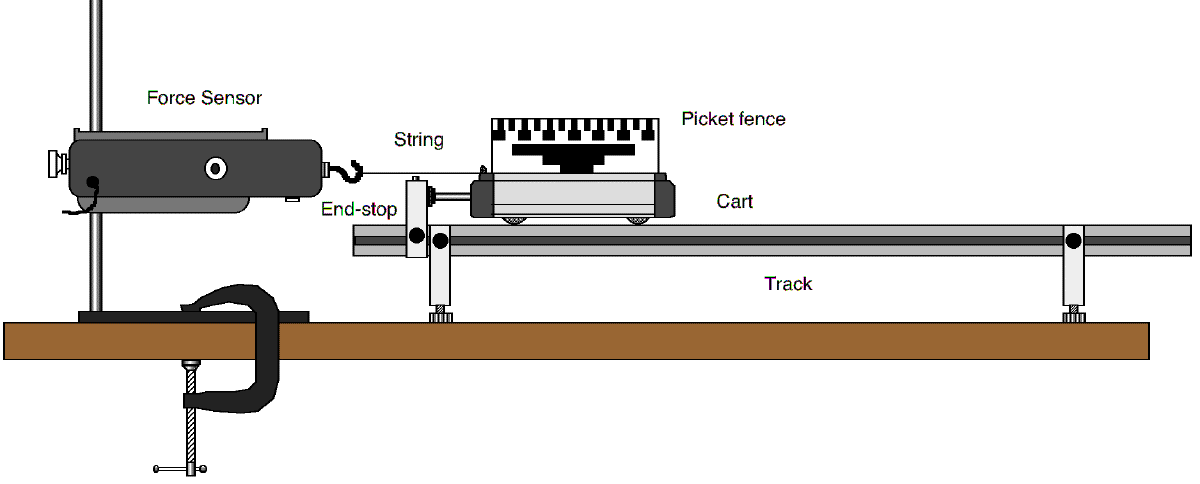
\includegraphics[width=\textwidth]{Energy_2_Prelab_Setup}
\end{enumerate}•

\subsubsection*{Pre-Lab Data Collection}
\begin{enumerate}
\item
Put the five-pattern picket fence in the accessory tray of the cart so that the pattern of 1 cm opaque bands is at the top.
\item
Measure the mass of the cart plus the picket fence. Record the mass in the data table.
\item
Place the cart so the end of its plunger bar is against the end stop. Tie one end of the string to the small hole in the end cap of the cart just above the plunger.
\item
Tie the other end of the string to the Force Sensor's hook.
\item
Slide the track itself away from the force sensor so the string is taut and the plunger is against the end stop but the plunger spring is \emph{not} compressed. Make a mark on the edge of the track to indicate the initial position of the end of the cart.
\item
In Capstone, next to the Record button click on the button labeled ``Continuous Mode" and change it to ``Keep Mode."
\item
Click on the Preview button to begin data sampling.
\item
Press the tare button on the side of the Force Sensor to zero the sensor.
\item
In the table, type in ``0" under the Compression column, then click on ``Keep" to store the present Force Sensor value.
\item \label{step:SpringConstant_start}
Slide the track away from the Force Sensor so the plunger spring is compressed 5 mm (0.005 m) against the end stop. Use the mark on the track as a reference guide. Make sure the string between the sensor and the cart is kept taut. \emph{Hold} the track in this new position.
\item \label{step:SpringConstant_end}
Enter ``0.005" into the table under Compression on the next row and click the Keep button to store the new value.
\item
Repeat steps~\ref{step:SpringConstant_start}--\ref{step:SpringConstant_end} moving the track away from the sensor in 5 mm increments until the plunger spring has been compressed 20 mm.
\item
Press the Stop button to finish data collection.
\end{enumerate}•

\subsubsection*{Pre-lab Analysis}
\begin{enumerate}
\item
Rescale the data in the graph as necessary.
\item
Apply a Linear Fit to the data. The slope of this line is the spring constant $k$ that we are looking for. Record this value in the data table.
\item
\textbf{Print} a copy of the table and graph for each member of the group.
\item
Remove the string from the Force Sensor's hook. Disconnect the Force Sensor and wrap the cord. Set the sensor aside.
\end{enumerate}•

Now, for the experiment itself we will use the Photogate to measure the motion of the cart just after it is pushed by the plunger spring as it relaxes. Using Capstone we can then calculate the initial velocity and maximum kinetic energy of the cart. Finally, we will be able to compare our measured kinetic energy against the calculated elastic potential energy.
\begin{enumerate}
\item
Setup the track, cart, and Photogate as shown below. Put the cart on the track so the end of the plunger bar is pressed against the end stop but the spring is not compressed. Position the Photogate so that it is as close as possible to the edge of the picket fence.

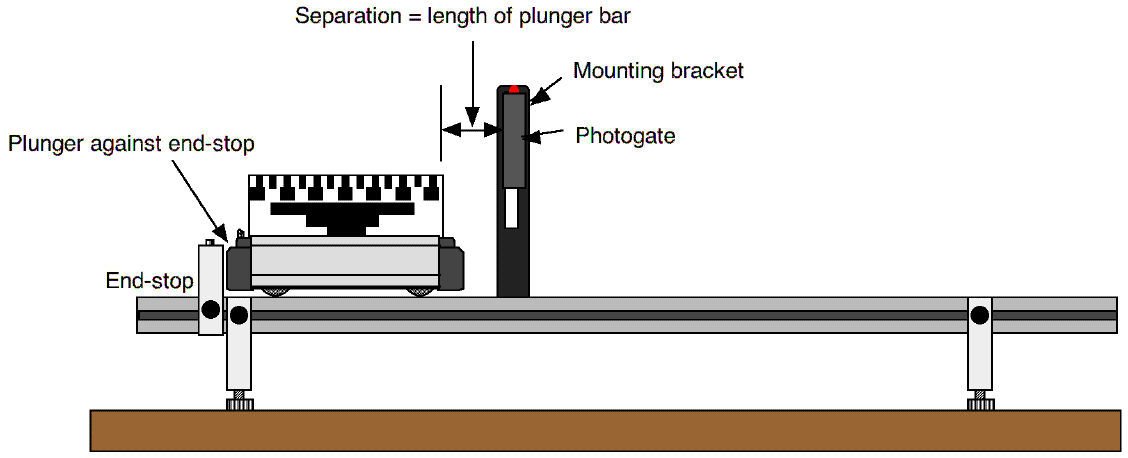
\includegraphics[width=\textwidth]{Energy_2_Experiment_Setup}

\item
Adjust the height of the Photogate so the beam will be blocked by the pattern of 1 cm opaque bands at the top edger of the picket fence.
\item
Connect the Photogate to the 850UI.
\item
Start a new experiment in Capstone 
\includegraphics{New_Experiment}. When prompted to save changes, choose ``Discard." 
\item
Under ``Hardware Setup" add the Photogate to the appropriate port.
\item
Click on ``Timer Setup" and choose ``Pre-Configured Timer" for the Photogate, Ch 1. 
\item	
Select ``Picket Fence," make sure that ``Speed" is checked.
\item
For the flag spacing make sure to change the value to 0.01 m.
\item
Click ``Next" then ``Finish." Finally, click on ``Timer Setup" again to hide the window.
\item
We now want to setup a calculated value of kinetic energy based on our velocity measurements of the cart. Click on ``Calculator" on the left.
\item
In the first line type ``Kinetic Energy = 0.5*mass*[Speed (m/s)]\^{}2" and give it units of ``J." (Once ``[" is typed we can simply select ``Speed" and Capstone will link the appropriate data set for the calculation.)
\item
The second line should now read ``mass =." Type in the mass (in kg) of the cart plus the picket fence into this line and give it units of ``kg."
\item
To make sure that our values are displayed properly, we will need to increase the display precision. To do this, click on the line containing our kinetic energy equation. Now, click on the properties button 
\includegraphics{Properties}. In the window that opens, under ``Numerical Format" increase the ``Number of Decimal Places" value to 3.
\item
Click on ``Calculator" again to hide the window.
\item
Double-click on ``Graph" in the toolbar on the right.
\item
Create a Speed vs. Time graph.
\item
Now to create a second plot below our Speed vs. Time graph, click on the ``Add New Plot Area" button 
\includegraphics{Add_New_Plot}. Select our ``Kinetic Energy (J)" calculation for the vertical axis on the bottom graph.
\end{enumerate}•

\subsection*{Procedure}
\begin{enumerate}
\item
Measure the length of the plunger relative to the end cap of the dynamics cart. Record the plunger length $x$ in the data table. n.b., When the cart is placed so the end of the plunger bar is pressed against the end stop, we can measure the length of the plunger by measuring the distance from the end stop to the cart.
\item \label{step:Energy2_start}
Completely compress the plunger spring on the cart and lock the spring in position by pushing the end of the plunger bar upward slightly so that one of its notches will catch on the metal rail inside the cart.
\item
Put the plunger end of the cart against the end stop. The separation between the edge of the picket fence furtherest away from the end stop and the Photogate should be the length of the plunger bar when the spring is not compressed.
\item
Click on the Record button to begin data collection.
\item
Use the end of a pencil or similar object to tap down on the plunger release button. The cart will be pushed away from the end stop by the plunger spring.
\item \label{step:Energy2_end}
Click on the Stop button to end data collection.
\item
Repeat steps~\ref{step:Energy2_start}--\ref{step:Energy2_end} two more times for a total of three runs.
\item
Add additional mass to the cart and update the mass in the calculator. Usually the slotted masses can fit under the picket fence block in the accessory tray of the cart. The Photogate height may need to be adjusted so that it is still blocked by the 1 cm opaque bands.  Record the mass of the cart, picket fence, and additional masses in the data table.
\item
Repeat steps~\ref{step:Energy2_start}--\ref{step:Energy2_end} three more times for a total of six runs altogether.
\end{enumerate}•

\subsection*{Analysis}
\begin{enumerate}
\item
Select Data Run \#1 by clicking on the ``Select Data Run" button 
\includegraphics{Select_Data_Run}.
\item
Click in the Kinetic Energy vs. Time graph.
\item
Using the Statistics button 
\includegraphics{Statistics}, display the Mean and Standard Deviation. Record these values in the data table.
\item
\textbf{Print} a copy of this graph for each group member.
\item \label{step:Energy2_Analysis}
Hide Run \# 1 and show Run \#2. Record the Mean and Standard Deviation in the data table.
\item
Repeat step~\ref{step:Energy2_Analysis} for each data run.
\item
Calculate the average kinetic energy from the results in the data table.
\item
Calculate the elastic potential energy using Equation~\eqref{eq:PE_Spring}.
\end{enumerate}•

\begin{question}
What is the percent difference between the average kinetic energy and the elastic potential energy? 
\end{question}
\begin{question}
Which energy was larger in each case, the elastic potential energy or the kinetic energy of the cart?
\end{question}
\begin{question}
What are possible reasons for the differences, if any?
\end{question}
\begin{question}
When the mass of the cart was increased, did the kinetic energy change? Should it change? Explain.
\end{question}
\begin{question}
How constant is the kinetic energy? (How does the standard deviation compare to the mean?) 
\end{question}

\begin{samepage}
\hrulefill\\ \\
\emph{Chapter~\ref{chap:Energy}:} \textbf{Energy}
\begin{enumerate}
\item
\textbf{(1)} Title Page
\item
\textbf{(3)} Purpose
\item
\textbf{(8)} Theory for Setup I (Work-Energy Theorem).
\item
\textbf{(4)} Procedure for Setup I. Hit the highpoints.
\item
\textbf{(4)} Data, Tables/Graphs, for both setups..
\item
\textbf{(22)} Answers to all questions.
\item
\textbf{(8)} Conclusion for Setup I. What were the goals of the experiment? Were they achieved? To within what error? Were there any major problems/errors? (n.b., human error is not an acceptable response. Be creative.) What could be done differently to improve or expand this experiment?
\end{enumerate}•
\end{samepage}

\newpage
\section{Data Tables}

\subsection*{Setup I}
\begin{doublespace}
\resizebox{0.8\textwidth}{!}{
\begin{tabular}{|l|@{\hskip 2 cm}r|}
\hline
Item & Value\\
\hline
Mass (cart \& sensor) & kg\\
\hline
$v_f$ (maximum) & m/s\\
\hline
$KE_{max}$ & J\\
\hline
Work ($F$ vs. $x$) & J\\
\hline
\end{tabular}•
}

\newpage
\subsection*{Setup II}
\resizebox{0.8\textwidth}{!}{
\begin{tabular}{|l|@{\hskip 2 cm}r|}
\hline
Item & Value\\
\hline
Mass (cart \& fence) & kg\\
\hline
Spring Constant $k$ & N/m\\
\hline
Plunger Length $x$ & m\\
\hline
Mass (cart, fence, \& extra mass) & kg\\
\hline
\end{tabular}•
}
\\[3 cm]
%\resizebox{0.8\textwidth}{!}{
\begin{tabular}{|l|@{\hskip 0.75 cm}l|@{\hskip 0.75 cm}l|@{\hskip 0.75 cm}l|@{\hskip 0.75 cm}l|@{\hskip 0.75 cm}l|@{\hskip 0.75 cm}l|@{\hskip 0.75 cm}l|}
\hline
Run \# & 1 & 2 & 3 & 4 & 5 & 6 & Average\\
\hline
KE (J) &&&&&&&\\
\hline
Std. Dev. (J)&&&&&&&\\
\hline
\end{tabular}•
%}

~
\\[1 cm]
Elastic Potential Energy = $PE_{elastic} = \frac{1}{2}kx^2=\rule[-1mm]{1.5cm}{.1pt}\text{ J}$
\end{doublespace}

\end{document}
